% Name: Recurrent network, unrolled
% Description: One recurrent cell drawn at three time steps, sharing the weights W between them.
% Tags: RNN, recurrent, sequence model

\usetikzlibrary{arrows.meta}

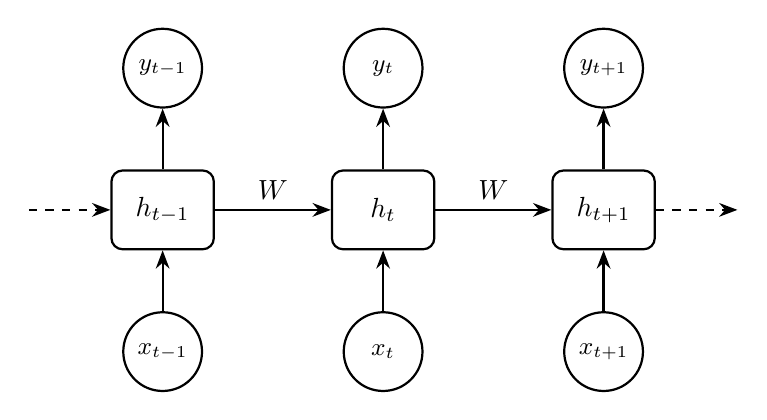
\begin{tikzpicture}[
  cell/.style={draw, thick, rounded corners, minimum width=13mm, minimum height=10mm},
  io/.style={circle, draw, thick, minimum size=10mm, inner sep=0pt, font=\small},
  arrow/.style={-{Stealth}, thick},
]
  \foreach \i/\t in {0/{t-1}, 1/t, 2/{t+1}} {
    \node[cell] (h\i) at (2.8*\i,0) {$h_{\t}$};
    \node[io] (x\i) at (2.8*\i,-1.8) {$x_{\t}$};
    \node[io] (y\i) at (2.8*\i,1.8) {$y_{\t}$};
    \draw[arrow] (x\i) -- (h\i);
    \draw[arrow] (h\i) -- (y\i);
  }
  \draw[arrow] (h0) -- node[above] {$W$} (h1);
  \draw[arrow] (h1) -- node[above] {$W$} (h2);
  \draw[arrow, dashed] (-1.7,0) -- (h0);
  \draw[arrow, dashed] (h2) -- (7.3,0);
\end{tikzpicture}
